\chapter{2019年「大学物理2」\titlelogo{https://sci.hdu.edu.cn}{HDU}期末试题}
\date{2020年2月20日}{大学物理教学团队}{A0715012}
{未央物理讲师 \href{https://qm.qq.com/q/UPbGudx8cK}{\textbf{Axia}}}
{https://h5.qun.qq.com/s/WRps3LNC8K}{HDU 物理营}
{http://weixin.qq.com/r/mhKYgFTEMQlOrRDj90eI}{未央学社公众号}

\section{选择题（每题3分，共27分）}

\begin{choice}{A}[弹簧振子]
一质量为$m$的滑块，两边分别与劲度系数为$k_1$和$k_2$的轻弹簧联接，两弹簧的另外两端分别固定在墙上．滑块$m$可在光滑的水平面上滑动，$O$点为系统平衡位置．将滑块$m$向右移动到$x_0$，自静止释放，并从释放时开始计时．取水平向右为正方向，则其振动方程为
\begin{tasks}(100)
    \task*(22) $x_0\cos\sqrt{\frac{k_1+k_2}{m}}t$
    \task*(24) $x_0\cos\sqrt{\frac{k_1k_2}{m\ab(k_1+k_2)}}t$
    \task*(24) $x_0\cos\sqrt{\frac{k_1+k_2}{m}}t+\pi$
    \task*(30) $x_0\cos\ab[\sqrt{\frac{k_1k_2}{m\ab(k_1+k_2)}}t+\pi]$
\end{tasks}
\end{choice}
\begin{solution}*
    两弹簧均连接在物块上且对物块的回复力方向相同，所以二者并联，系统角频率$\omega^2=\frac{k_1+k_2}{m}$.初始时刻$x=x_0,\ v<0$，所以初相$\varphi=0$，物块的运动方程为$x=x_0\cos{\ab(\sqrt{\frac{k_1+k_2}{m}}t)}$.\sokka{A}
\end{solution}

\vskip-2ex
\begin{paracol}{2}
    \begin{choice}{D}[平面简谐波]
        图为沿$x$轴负方向传播的平面简谐波在$t=0$时刻的波形．若波的表达式以余弦函数表示，则$O$点处质点振动的初相为
    \begin{tasks}(4)
        \task $0$
        \task $\frac{1}{2}\pi$
        \task $\pi$
        \task $\frac{3}{2}\pi$
    \end{tasks}
    \end{choice}
    \switchcolumn\centering
    \vfill
    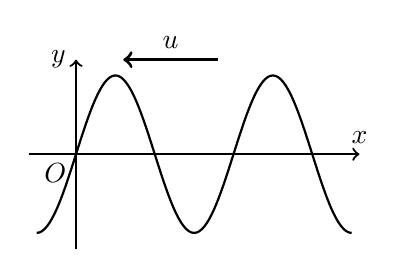
\begin{tikzpicture}
        \draw [thick,->] (-0.6,0)--(3.6,0) node [anchor=south] {$x$};
        \draw [thick,->] (0,-1.2)--(0,1.2) node [anchor=east] at (0,1.2) {$y$};
        \draw [thick] (-0.5,-1) cos (0,0) sin (0.5,1) cos (1,0) sin (1.5,-1) cos (2,0) sin (2.5,1) cos (3,0) sin (3.5,-1);
        \node [anchor=north east] at (0,0) {$O$};
        \draw [very thick,<-] (0.6,1.2)--(1.8,1.2) node [anchor=south,midway] {$u$};
    \end{tikzpicture}
    \vfill
\end{paracol}
\vspace{-.75em}
\begin{solution}*
    此时$O$点的振动速度大于零，所以$\varphi=-\frac{1}{2}\pi=\frac{3}{2}\pi$.\sokka{D}
\end{solution}

\begin{choice}{B}[驻波]
    在波长为$\lambda$的驻波中，两个相邻波腹之间的距离为
    \begin{tasks}(4)
        \task $\frac{\lambda}{4}$
        \task $\frac{\lambda}{2}$
        \task $\frac{3\lambda}{4}$
        \task $\lambda$
    \end{tasks}
\end{choice}

\vskip-2ex
\begin{paracol}{2}
    \begin{choice}{B}[弗琅禾费衍射]
        一束波长为$\lambda$的平行单色光垂直入射到一单缝$AB$上，装置如图.在屏幕$D$上形成衍射图样，如果$P$是一级暗纹所在的位置，则$\overline{BC}$的长度为
    \begin{tasks}(4)
        \task $\frac{\lambda}{2}$
        \task $\lambda$
        \task $\frac{3\lambda}{2}$
        \task $2\lambda$
    \end{tasks}
    \end{choice}
    \switchcolumn\centering
\vfill
\begin{tikzpicture}[scale=.9]
    \filldraw [fill=gray] (0.2,1.5) rectangle (0,0.5) node [anchor=south east] {$A$};
    \filldraw [fill=gray] (0.2,-1.5) rectangle (0,-0.5) node [anchor=north east] {$B$};
    \draw [thick,dashed] (-1.2,0)--(3.6,0);
    \draw [thick] (3.6,1.5)--(3.6,-1.5) node [anchor=west,at start] {$D$} node [anchor=west] {屏};
    \filldraw [fill=backgroundcolor] (1.5,0) ellipse (0.1 and 1.2);
    \foreach \y in {0.5,0,-0.5}
    \draw [thick,->,yshift=\y cm] (-1,0)--(0,0);
    \length{(1.5,-1.4)}{(3.6,-1.4)}{$f$}{(0.25,0)}
    \node [anchor=south] at (-1,0.5) {$\lambda$};
    \node [anchor=south] at (1.5,1.2) {$L$};
    \draw [thick] (0,0.5)--(1.5,1)--(3.6,1);
    \draw [thick] (0,0)--(1.5,0.5)--(3.6,1);
    \draw [thick] (0,-0.5)--(1.5,0)--(3.6,1) node [anchor=west] {$P$};
    \draw [dashed] (0,-0.5)--(0,0.5)--(0.32,-0.4) node [anchor=north west] {$C$};
\end{tikzpicture}
\vfill
\end{paracol}
\vspace{-.75em}
\begin{solution}*
    由暗纹条件$\overline{BC}=\delta=1\cdot\lambda$.\sokka{B}
\end{solution}

\begin{choice}{C}[光的偏振]
使一光强为$I_0$的平面偏振光先后通过两个偏振片$P_1$和$P_2$. $P_1$和$P_2$的偏振化方向与原入射光光矢量振动方向的夹角分别是$\alpha$和$90^{\circ}$，则通过这两个偏振片后的光强$I$是
\begin{tasks}(4)
    \task $\frac{1}{2}I_0\cos^2{\alpha}$
    \task $0$
    \task $\frac{1}{4}I_0\sin^2\ab(2\alpha)$
    \task $\frac{1}{4}I_0\sin^2{\alpha}$
\end{tasks}
\end{choice}
\solute0
\begin{solution}*
    由Malus定律得$I=I_0\cos^2{\alpha}\cos^2{\ab(\frac{\pi}{2}-\alpha)}=\frac{1}{4}I_0\sin^2{\ab(2\alpha)}$.\sokka{C}
\end{solution}

\begin{choice}{D}[相对论基本原理]
有下列几种说法
\begin{tasks}(2)
    \task[(1)] 所有惯性系对物理基本规律都是等价的
    \task[(2)] 在真空中光度与光的频率、光源的运动状态无关
    \task*[(3)] 在任何惯性系中，光在真空中沿任何方向的传播速率都相同
\end{tasks}

其中说法正确的是
\begin{tasks}(4)
    \task (1)(2)
    \task (1)(3)
    \task (2)(3)
    \task (1)(2)(3)
\end{tasks}
\end{choice}
\begin{solution}*
    由相对性原理和光速不变原理可知三个说法都是正确的.\sokka{D}
\end{solution}

\begin{choice}{C}[尺缩效应]
    一宇航员要到离地球为5光年的星球. 如果宇航员希望把路程缩短为3光年，则他所乘的火箭相对于地球的速度应是
\begin{tasks}(4)
    \task $\frac{1}{2}c$
    \task $\frac{3}{5}c$
    \task $\frac{4}{5}c$
    \task $\frac{9}{10}c$
\end{tasks}
\end{choice}
\solute0
\begin{solution}*
    由尺缩效应$3\mathrm{ly}=5\mathrm{ly}\sqrt{1-v^2/c^2}$得$v=0.8\mathrm{c}$.\sokka{C}
\end{solution}

\begin{choice}{C}[四个量子数]
    在原子的L壳层中，电子可能具有的四个量子数$(n,l,m_l,m_s)$是
\begin{tasks}[label=\roman*.](4)
    \task $(2,0,1,\frac{1}{2})$
    \task $(2,1,0,-\frac{1}{2})$
    \task $(2,1,1,\frac{1}{2})$
    \task $(2,1,-1,-\frac{1}{2})$
\end{tasks}
\begin{tasks}(4)
    \task 只有i, ii是正确的
    \task 只有ii, iii是正确的
    \task 只有ii, iii, iv是正确的
    \task 全部是正确的
\end{tasks}
\end{choice}
\solute0
\begin{solution}*
    四个量子数：$n$确定时，$l=0,\pm 1,\cdots,\pm n-1;\ m_l=0,\pm 1,\cdots,\pm l;\ m_s=\pm1/2$.\sokka{C}
\end{solution}

\begin{choice}{B}[光电效应]
以一定频率的单色光照射在某种金属上，测出其光电流曲线在图中用实线表示，然后保持光的频率不变，增大照射光的强度，测出其光电流曲线在图中用虚线表示.满足题意的图是
\vskip2ex
\centering
\begin{tikzpicture}[scale=0.6]
    \foreach \a in {0,7.5,15,22.5}
    {
    \draw [->,xshift=\a cm] (-1,0)--(3,0) node [anchor=south] {$U$} node [anchor=north east,near start] {$O$};
    \draw [->,xshift=\a cm] (0,-0.5)--(0,3) node [anchor=west] {$I$};
    \draw [xshift=\a cm,] (-0.6,0)..controls (0.6,0.5) and (-0.6,1.8)..(2.5,2.1);
    }
    \draw [dashed] (-0.6,0)..controls (0.9,0.8) and (-0.6,1.8)..(2.8,2.3);
    \draw [xshift=7.5 cm,dashed] (-0.6,0)..controls (0.3,2.4) ..(2.5,2.4);
    \draw [xshift=15cm,dashed] (-0.6,0)..controls (0.5,2.1) and (-0.5,1.6) ..(2.5,2.1);
    \draw [xshift=22.5cm,dashed] (-0.3,0)..controls (1.5,0.8) and (0.3,2.2) ..(2.5,2.4);
    \node [anchor=north] at (1.5,-0.5) {A};
    \node [anchor=north] at (9,-0.5) {B};
    \node [anchor=north] at (16.5,-0.5) {C};
    \node [anchor=north] at (24,-0.5) {D};
\end{tikzpicture}
\end{choice}

\section{填空题（共21分）}
\begin{problem}[弹簧振子][3]
    一物块悬挂在弹簧下方做简谐振动，当这物块的位移等于振幅的一半时，其动能是总能量的\ans{$3/4$}（设平衡位置处势能为零）.当这物块在平衡位置时，弹簧的长度比原长长$\Delta l$，这一振动系统的周期为\ans{$2\pi\sqrt{\Delta l/g}$}.
\end{problem}
\begin{solution}*
    此时物块动能为$E_k=\frac{1}{2}kA^2-\frac{1}{2}k\ab(\frac{A}{2})^2=\frac{3}{4}\cdot\frac{1}{2}kA^2$，所以此时物块动能是总能量的$\frac{\frac{3}{4}\cdot\frac{1}{2}kA^2}{\frac{1}{2}kA^2}=\frac{3}{4}$；弹簧的劲度系数$k=\frac{mg}{\Delta l}$，由弹簧振子周期表达式得系统的周期为$T=2\pi\sqrt{\frac{m}{k}}=2\pi\sqrt{\frac{\Delta l}{g}}$.
\end{solution}

\begin{problem}[驻波][3]
    设入射波的表达式为$y_1=A\cos\ab[2\pi\ab(\nu t+\frac{x}{\lambda})+\pi]$，波在$x=0$处发生反射，反射点为一固定端，则入射波和反射波合成的驻波的波腹位置所在处的坐标为\ans{$\frac{k\lambda}{2},\ k=0,1,2\cdots$}.
\end{problem}
\begin{solution}*
    反射波的表达式为$y_2=A\cos{\ab[2\pi\ab(\nu T-\frac{x}{\lambda})]}$，由此得驻波表达式$y_1+y_2=2A\cos{\ab(2\pi\nu T)}\cos{\ab(\frac{2\pi x}{\lambda})}$，所以波腹的位置为$\cos{\ab(\frac{2\pi x}{\lambda}-\frac{\pi}{2})}=\pm 1,\ x=\frac{k\lambda}{2},\ k=0,1,2\cdots$.
\end{solution}

\vskip-2ex
\begin{paracol}{2}
    \begin{problem}[光程和光程差][3]
        如图所示，两缝$S_1$和$S_2$之间的距离为$d$，媒质的折射率为$n=1$，平行单色光斜入射到双缝上，入射角为$\theta$则屏幕上$P$处，两相干光的光程差为\ans{$r_2-r_1-d\sin{\theta}$}.
    \end{problem}
    \switchcolumn\centering
    \vfill
    \begin{tikzpicture}[scale=0.48]
        \draw [dash dot] (-0.2,0)--(6.2,0) node [anchor=west] {{$O$}};
        \draw (0,1.5)--(0,3);
        \draw (0,-1)--(0,1);
        \draw (0,-1.5)--(0,-3);
        \draw [2号色,thick] (0,1.25)--(6,2.25) node [midway,anchor=south] {$r_1$};
        \draw [2号色,thick] (0,-1.25)--(6,2.25) node [midway,anchor=south] {$r_2$} node [anchor=west] {$P$};
        \draw (6,3)--(6,-3);
        \node [anchor=south west] at (0,1.25) {$S_1$} node [anchor=north west] at (0,-1.25) {$S_2$};
        \length{(0.5,1.25)}{(0.5,-1.25)}{$d$}{(0,-0.75)}
        \draw[->] (-1.7,0.75) --(-0.2,1.25);
        \draw[->] (-1.7,-1.75)--(-0.2,-1.25) node [near start,anchor=south] {{$\lambda$}};
        \draw [dashed] (0,1.25)--(-1.5,1.25);
        \coordinate (b) at (-1.75,0.75);
        \coordinate (a) at (0,1.25);
        \coordinate (c) at (-1.5,1.25);
        \pic["\footnotesize$\theta$",draw=black, thick, angle eccentricity=1.25, angle radius=20]{angle=c--a--b};
    \end{tikzpicture}
    \vfill
\end{paracol}
\vspace{-.75em}

\begin{problem}[起偏角][3]
    一束自然光入射到折射率分别为$n_1$和$n_2$的两种介质的交界面上，发生反射和折射.已知反射光是完全偏振光，那么折射角$r$的值为\ans{$\frac{\pi}{2}-\arctan{\frac{n_2}{n_1}}$}.
\end{problem}
\begin{solution}*
    起偏角为$\arctan{\frac{n_2}{n_1}}$，由起偏条件$i+r=90^{\circ}$得折射角$r=\frac{\pi}{2}-\arctan{\frac{n_2}{n_1}}$.
\end{solution}

\begin{problem}[钟慢效应][3]
    $\pi^+$介子是不稳定的粒子，在它自己的参照系中测得平均寿命是$2.6\times 10^{-8}\mathrm{s}$，如果它相对于实验室以$0.8c$的速率运动，那么实验室坐标系中测得的$\pi^+$介子的寿命是\ans{$4.33\times 10^{-8}\mathrm{s}$}.
\end{problem}
\begin{solution}*
    由钟慢效应公式$t=\frac{t_0}{\sqrt{1-\beta^2}}=4.33\times 10^{-8}\mathrm{s}$.
\end{solution}

\begin{problem}[相对论能动量关系][3]
    设电子静止质量为$m_e$，将一个电子从静止加速到速率为$0.6c$，需做功\ans{$\frac{1}{4}m_ec^2$}.
\end{problem}
\begin{solution}*
    $W=mc^2-m_0c^2=\frac{m_e}{\sqrt{1-v^2/c^2}}-m_ec^2=\frac{1}{4}m_ec^2$
\end{solution}

\begin{problem}[壳层结构][3]
    多电子原子中，电子的排列遵循\ans{泡利不相容}原理和\ans{能量最低}原理．
\end{problem}

\section{计算题（共52分）}
\begin{paracol}{2}
\begin{problem}[简谐振动][6]
    一简谐振动的振动曲线如图所示，求振动方程.
\end{problem}
\vspace{-.75em}
\solute3
\begin{solution}*
    \begin{itemize}
        \item $t=0$时，$x=-5\mathrm{cm},\ v<0$，所以初相$\varphi=2\pi/3$.\point{2}
        \item $t=2$时相位$\varphi=-\frac{\pi}{2}=\omega\cdot 2+\frac{2\pi}{3}$，得角频率$\omega=\frac{5}{12}\pi$.\point{2}
        \item 综上，振动方程为$y=0.1\cos{\ab(\frac{5}{12}\pi t+\frac{2\pi}{3})}$.\point{2}
    \end{itemize}
\end{solution}
\switchcolumn\centering
\vfill
\begin{tikzpicture}[scale=1.2]
        \draw [->,thick] (-0.5,0)--(3.6,0) node [anchor=south] {$t$};
        \draw [->,thick] (0,-1.5)--(0,1.5) node [anchor=west] {$x$};
        \draw[thick,H1] (0,-0.5) sin (0.4,-1) cos (1,0) sin (1.6,1) cos (2.2,0) sin (2.8,-1) cos (3.4,0);
        \draw [densely dashed] (0,1)--(1.6,1);
        \node [anchor=east] at (0,1) {$10$} node [anchor=south east] at (0,0) {$O$} node [anchor=east] at (0,-0.5) {$-5$} node [anchor=east] at (0,-1) {$-10$} node [anchor=south east] at (1,0) {$2$};
    \end{tikzpicture}
\vfill
\end{paracol}

\vskip-2ex
\begin{paracol}{2}
\begin{problem}[平面简谐波的波函数][6]
        如图所示，一简谐波向$x$轴正向传播，波速$u=500\mathrm{m/s},\ x_0=1\mathrm{m}$处$P$点的振动方程为$y=0.03\cos{\ab(500\pi t-\frac{\pi}{2})}$ (SI).
    \begin{enumerate}
        \item 按图所示坐标系，写出相应的波的表达式.
        \item 在图上画出$t=0$时刻的波形曲线.
    \end{enumerate}
\end{problem}
\vspace{-.75em}
\solute1
\begin{solution}*
    $y\ab(x,t)=0.03\cos{\ab[500\pi\ab(t-\frac{x-1}{500})-\frac{1}{2}\pi]}$ (SI).
\end{solution}
\switchcolumn\centering
\vfill
\begin{tikzpicture}[scale=0.83]
    \draw [->] (-2,0)--(4,0) node [anchor=north] {$x/\mathrm{m}$};
    \draw [->] (0,-1.5)--(0,2) node [anchor=west] {$y/\mathrm{m}$};
    \length{(0,-0.5)}{(1.5,-0.5)}{$x_0$}{(0.5,0)}
    \draw [->] (1.5,1.5)--(2.5,1.5) node [midway,anchor=south] {$u$};
    \node at (2.5,1){\footnotesize$y\ab(x,0)=0.03\cos{\ab(\pi x-\frac{\pi}{2})}$};
    \draw [very thick,solutioncolor] (-1.5,0) sin (-0.75,-0.5) cos (0,0) sin (0.75,0.5) cos (1.5,0) sin (2.25,-0.5) cos (3,0) sin (3.75,0.5);
    \draw [dashed] (0,0.5)--(0.75,0.5) node [at start,anchor=east] {$0.03$};
\end{tikzpicture}
\vfill
\end{paracol}

\vspace{-.75em}
\begin{problem}[劈尖干涉][5]
    用波长为$\lambda=500\mathrm{nm}$的单色光垂直照射折射率$n=1.33$的劈尖膜观察反射光的等厚干涉.从劈尖膜的棱算起，第五条明纹中心对应的膜厚是多少.
\end{problem}
\solute0
\begin{solution}*
    由明纹条件$\delta=2nh+\lambda/2=k\lambda$得$k=5$时，$h=9\lambda/4n=0.85\mu\mathrm{m}$.
\end{solution}

\begin{problem}[弗琅禾费衍射][10]
\begin{enumerate}
    \item 在单缝夫琅禾费衍射实验中，垂直入射的光有两种波长，$\lambda_1=400\mathrm{nm}\ \lambda_2=760\mathrm{nm}$.已知单缝宽度$a=1.0\times 10^{-2}\mathrm{cm}$，透镜焦距$f=50\mathrm{cm}$.求两种光第一级衍射明纹中心之间的距离.
    \item 若用光栅常数$d=1.0\times10^{-3}\mathrm{cm}$的光栅替换单缝，其他条件和上一问相同，求两种光第一级主极大之间的距离.
\end{enumerate}
\end{problem}
\solute1
\begin{solution}
    \begin{enumerate}
        \item 由单缝衍射明纹公式$a\sin{\varphi}=\frac{2k+1}{2}\lambda\approx\frac{xa}{f}$得一级明纹间距$\Delta x=x_2-x_1=\frac{3\ab(\lambda_2-\lambda_1)f}{2a}=0.27\mathrm{cm}$.\point{5}
        \item 由光栅主极大公式$d\sin\varphi=k\lambda\approx\frac{x}{f}$得两个主极大之间距离
        $\Delta x=x_2-x_1=\frac{\ab(\lambda_2-\lambda_1)f}{d}=1.8\mathrm{cm}$\point{5}
    \end{enumerate}
\end{solution}

\begin{problem}[光的偏振][8]
    将两个偏振片叠放在一起，此两偏振片的偏振化方向之间的夹角为，一束光强为$I_0$的线偏振光垂直入射到偏振片上，该光束的光矢量振动方向与二偏振片的偏振化方向皆成$30^{\circ}$角.
\begin{enumerate}
    \item 求透过每个偏振片后的光束强度.
    \item 若将原入射光束换为强度相同的自然光，求透过每个偏振片后的光束强度.
\end{enumerate}
\end{problem}
\solute0
\begin{solution}
\begin{enumerate}
    \item 线偏光透过偏振片1后与偏振片2夹角为$60^{\circ}$.由Malus定律得$I_1=I_0\cos^2{30^{\circ}}\cos^2{60^{\circ}}=\frac{3}{16}I_0$.\point{4}
    \item 自然光透过偏振片1后光强减半，与偏振片2夹角为$60^{\circ}$.由Malus定律得$I_2=\frac{1}{2}I_0\cos^2{60^{\circ}}=\frac{1}{8}I_0$.\point{4}
\end{enumerate}
\end{solution}

\begin{problem}[相对论能动量关系][6]
    一电子（静质量$m_e=9.11\times 10^{-31}\mathrm{kg}$）以$0.99c$的速率运动，试求
\begin{enumerate}
    \item 电子的总能量.
    \item 电子的经典力学的动能与相对论动能之比.
\end{enumerate}
\end{problem}
\begin{solution}*
    $E=m_c^2=\frac{m_ec^2}{\sqrt{1-\beta^2}}=5.8\times 10^{-13}\mathrm{J}$，$\frac{E_{k_0}}{E_k}=\frac{\frac{1}{2}m_ev^2}{m_c^2-m_ec^2}=8.13\%$.
\end{solution}

\begin{multicols*}{2}
\begin{problem}[光电效应][6]
    光电管的阴极用逸出功$A=2.2e\mathrm{V}$的金属制成，今用一单色光照射此光电管，阴极发射出光电子，测得遏止电势差为$\abs{U_a}=5.0e\mathrm{V}$.试求
\begin{enumerate}
    \item 光电管的阴极金属的光电效应红限波长.
    \item 入射光波长.
\end{enumerate}
\end{problem}
\begin{solution}
\begin{enumerate}
    \item $\lambda_{\max}=hc/A=563.56\mathrm{nm}$.\point{3}
    \item $\lambda=hc/(eU_a+A)=172.20\mathrm{nm}$.\point{3}
\end{enumerate}
\end{solution}
\begin{problem}[][5]
    无限深势阱中运动粒子波函数为$\psi\ab(x)=\sqrt{\frac{2}{a}}\sin\ab(\frac{\pi x}{a})$，求发现粒子的概率密度为最大的位置 $(0\leq x\leq a)$.
\end{problem}
\solute2
\begin{solution}
粒子的概率密度为
\[\omega=\abs{\psi(x)}^2=\frac2a\sin^2\ab(\frac{\pi x}{a})\]
    令$\frac{\d\omega}{\d x}=0$得在$0\leq x\leq a$范围内发现粒子的概率密度为最大位置为$x=a/2$. 
\end{solution}
\end{multicols*}